\documentclass[12pt,a4paper]{article}

% ── Packages ──────────────────────────────────────────────────────────────────
\usepackage[utf8]{inputenc}
\usepackage[T1]{fontenc}
\usepackage[english]{babel}
% microtype omitted for compatibility
\usepackage{geometry}
\geometry{margin=2.5cm}

\usepackage{graphicx}
\usepackage{hyperref}
\hypersetup{colorlinks=true, linkcolor=blue, urlcolor=blue, citecolor=blue}
\usepackage{booktabs}
\usepackage{longtable}
\usepackage{caption}
\usepackage{listings}
\usepackage{xcolor}
\usepackage{amsmath}
\usepackage{enumitem}
\usepackage{titlesec}
\usepackage{abstract}
\usepackage{fancyhdr}
\usepackage{setspace}
\usepackage{float}

% ── SPARQL / Code style ────────────────────────────────────────────────────────
\definecolor{sparqlkeyword}{RGB}{0,0,180}
\definecolor{sparqlstring}{RGB}{160,32,32}
\definecolor{sparqlcomment}{RGB}{80,120,80}
\definecolor{sparqlbg}{RGB}{248,248,248}
\definecolor{sparqlborder}{RGB}{200,200,200}

\lstdefinelanguage{SPARQL}{
  morekeywords={SELECT, DISTINCT, WHERE, PREFIX, SERVICE, FILTER, OPTIONAL,
                UNION, LIMIT, OFFSET, ORDER, BY, ASC, DESC, CONSTRUCT, ASK,
                FROM, NAMED, GRAPH, GROUP, HAVING, VALUES, BIND, AS,
                isIRI, isLiteral, isBlank, str, lang, datatype, REGEX,
                STR, LANG, DATATYPE, BOUND, NOW, YEAR, MONTH, DAY,
                HOURS, MINUTES, SECONDS, TIMEZONE, TZ, MD5, SHA1, SHA256,
                SHA384, SHA512, IRI, URI, BNODE, STRDT, STRLANG, a},
  sensitive=true,
  morecomment=[l]{\#},
  morestring=[b]",
  morestring=[b]'
}

\lstset{
  language=SPARQL,
  basicstyle=\ttfamily\small,
  keywordstyle=\color{sparqlkeyword}\bfseries,
  stringstyle=\color{sparqlstring},
  commentstyle=\color{sparqlcomment}\itshape,
  backgroundcolor=\color{sparqlbg},
  frame=single,
  rulecolor=\color{sparqlborder},
  breaklines=true,
  breakatwhitespace=false,
  tabsize=2,
  captionpos=b,
  numbers=left,
  numberstyle=\tiny\color{gray},
  numbersep=8pt,
  showstringspaces=false,
  xleftmargin=1.5em,
  framexleftmargin=1.5em
}

% ── Header / Footer ────────────────────────────────────────────────────────────
\pagestyle{fancy}
\fancyhf{}
\rhead{Query Answering over Linked Data}
\lhead{BINDA R. \& WAHARTE M.}
\cfoot{\thepage}

% ── Title ──────────────────────────────────────────────────────────────────────
\title{
  \Large \textbf{Query Answering over Linked Data}\\[0.4em]
  \large Project Report --- Semantic Web
}
\author{
  Raphaël \textsc{Binda} \and Mathieu \textsc{Waharte}
}
\date{May 2026}

% ══════════════════════════════════════════════════════════════════════════════
\begin{document}

\maketitle
\thispagestyle{fancy}

% ── Abstract ──────────────────────────────────────────────────────────────────
\begin{abstract}
This report explores query answering over Linked Data using SPARQL and federated
queries across publicly available knowledge graphs.
We first demonstrate the expressive power of the Semantic Web stack by answering
a biomedical question (proteins involved in signal transduction and related to
pyramidal neurons) that cannot be handled by large language models alone due to
their lack of real-time, structured biological data.
We then propose and answer a complex geopolitical question about COVID-19 vaccine
developers using Wikidata.
Finally, we discuss how \texttt{CONSTRUCT} queries provide formal justification
for Linked Data answers, and how hybrid Linked Data / LLM pipelines combine the
complementary strengths of both paradigms.
\end{abstract}

\vspace{0.5em}
\noindent\rule{\linewidth}{0.4pt}
\tableofcontents
\vspace{1em}

% ══════════════════════════════════════════════════════════════════════════════
\newpage
\section{Introduction}
\label{sec:intro}

The World Wide Web, originally designed for human consumption, has evolved
towards a machine-readable layer known as the \emph{Semantic Web} or
\emph{Web of Data}~\cite{bernerslee2001}.
At its core, the Semantic Web relies on the Resource Description Framework
(RDF) to express knowledge as triples (\emph{subject--predicate--object}),
and on SPARQL as the standard query language to retrieve and manipulate that
knowledge.
The Linked Open Data (LOD) cloud~\cite{lodcloud} today contains billions of
such triples distributed across hundreds of interconnected datasets, covering
domains from biomedicine (UniProt, Bgee, LinkedLifeData) to culture and
encyclopaedic knowledge (DBpedia, Wikidata).

In his 2009 TED talk, Tim Berners-Lee challenged the scientific community to
unlock the potential of Linked Data for answering complex, cross-domain
questions~\cite{tbl2009}.
One such question --- ``\textit{What proteins are involved in signal
transduction and also related to pyramidal neurons?}'' --- illustrates
precisely why the Semantic Web is indispensable: it requires joining
heterogeneous, specialised databases in a single, structured, reproducible
query, something that Large Language Models (LLMs) alone cannot reliably do.

This project addresses three tasks:
\begin{enumerate}[label=\textbf{Q\arabic*.}]
  \item Demonstrate a Semantic Web method to answer the above biomedical
        question using federated SPARQL.
  \item Propose and answer a new complex question --- which organisations
        developed COVID-19 vaccines, and in which countries are they based? ---
        using Wikidata.
  \item Explain and justify the answers using \texttt{CONSTRUCT} queries and
        discuss a hybrid Linked Data + LLM approach.
\end{enumerate}

% ══════════════════════════════════════════════════════════════════════════════
\newpage
\section{Problem Statement}
\label{sec:problem}

Answering complex factual questions requires three capabilities that simple
keyword search or LLMs lack: (i)~\textbf{access to up-to-date, structured
data}, (ii)~\textbf{the ability to join information across heterogeneous
sources}, and (iii)~\textbf{provenance and justification} of the answer.

LLMs like ChatGPT encode world knowledge statically at training time. They
cannot query live databases, cannot guarantee that their answers reflect the
current state of specialised repositories (e.g.\ UniProt protein annotations),
and cannot easily provide a formal justification (a \emph{proof}) of how an
answer was derived from source data.

The Semantic Web stack --- RDF, OWL, SPARQL, and the federated query
mechanism introduced in SPARQL~1.1 --- directly addresses these limitations.
The challenge is to translate natural-language questions into correct SPARQL
queries, navigate the data models of multiple endpoints, and combine the results
coherently.

% ══════════════════════════════════════════════════════════════════════════════
\newpage
\section{Question 1 --- Biomedical Federated Query}
\label{sec:q1}

\subsection{Question}

\begin{quote}
\textit{What proteins are involved in signal transduction and also related to
pyramidal neurons?}
\end{quote}

This question was posed by Tim Berners-Lee in his 2009 TED talk as an example
of a query that could, in principle, be answered by connecting biological
databases on the Web, but that was not yet tractable at the time.

\subsection{Datasets explored}

\begin{itemize}
  \item \textbf{UniProt} (\url{https://sparql.uniprot.org/sparql}): the
        reference database for protein sequences and functional annotation.
        Each protein can be annotated with Gene Ontology (GO) terms, including
        GO:0007165 (\emph{signal transduction}).
  \item \textbf{Bgee} (\url{https://www.bgee.org/sparql}): a database of gene
        expression across anatomical entities and developmental stages.
        It provides expression data for genes in specific cell types such as
        pyramidal neurons.
  \item \textbf{Gene Ontology (OBO)} (\url{https://purl.obolibrary.org/obo/}):
        the controlled vocabulary linking biological processes to GO terms,
        used to navigate the hierarchy of signal transduction subprocesses.
\end{itemize}

\subsection{Method}

The key insight is that the two conditions in the question are held in
\emph{different} databases:
\begin{enumerate}
  \item Signal transduction annotation lives in UniProt (via GO terms).
  \item Expression in pyramidal neurons lives in Bgee (via anatomical entity
        labels).
\end{enumerate}

SPARQL~1.1's \texttt{SERVICE} keyword enables federated queries: a single
SPARQL query can delegate sub-queries to remote endpoints and join the results
locally. The bridge between the two databases is the UniProt identifier, which
Bgee exposes through the \texttt{lscr:xrefUniprot} predicate.

\subsection{SPARQL Query}

\begin{lstlisting}[caption={Federated SPARQL query joining UniProt and Bgee.},
                   label={lst:q1}]
PREFIX up:    <http://purl.uniprot.org/core/>
PREFIX go:    <http://purl.obolibrary.org/obo/>
PREFIX lscr:  <http://purl.org/lscr#>
PREFIX genex: <http://purl.org/genex#>
PREFIX orth:  <http://purl.org/net/orth#>
PREFIX rdfs:  <http://www.w3.org/2000/01/rdf-schema#>

SELECT DISTINCT ?protein ?proteinName ?goTerm ?goLabel WHERE {

  # Condition 1: Protein involved in signal transduction (UniProt)
  SERVICE <https://sparql.uniprot.org/sparql> {
    ?protein a up:Protein ;
             up:recommendedName/up:fullName ?proteinName ;
             up:classifiedWith ?goTerm .
    ?goTerm rdfs:subClassOf* go:GO_0007165 .  # signal transduction
    ?goTerm rdfs:label ?goLabel .
  }

  # Condition 2: Gene expressed in pyramidal neurons (Bgee)
  SERVICE <https://www.bgee.org/sparql> {
    ?gene a orth:Gene ;
          genex:isExpressedIn ?cond .
    ?cond genex:hasAnatomicalEntity ?anatEntity .
    ?anatEntity rdfs:label "pyramidal neuron"@en .
    ?gene lscr:xrefUniprot ?protein .
  }
}
\end{lstlisting}

\subsection{Difficulties encountered}

\begin{itemize}
  \item \textbf{Data model exploration}: the predicate connecting a protein to
        an anatomical entity is not obvious. We first had to inspect the Bgee
        ontology to discover the \texttt{genex:isExpressedIn} / 
        \texttt{genex:hasAnatomicalEntity} chain.
  \item \textbf{GO hierarchy}: signal transduction has many sub-processes.
        Using \texttt{rdfs:subClassOf*} (transitive closure) correctly captures
        all relevant GO terms without hardcoding each one.
  \item \textbf{Cross-database identifier alignment}: UniProt protein URIs must
        match Bgee's \texttt{lscr:xrefUniprot} values. This required checking
        that both sides use the canonical UniProt accession format.
  \item \textbf{Endpoint availability}: federated queries depend on remote
        endpoints being online and responsive; timeouts can occur for broad
        queries.
\end{itemize}

% ══════════════════════════════════════════════════════════════════════════════
\newpage
\section{Question 2 --- COVID-19 Vaccines and Their Developers}
\label{sec:q2}

\subsection{Question}

\begin{quote}
\textit{Which COVID-19 vaccines were developed by which organisations, and
in which country are those organisations based?}
\end{quote}

\subsection{Datasets explored}

\textbf{Wikidata} (\url{https://query.wikidata.org}) was chosen as the primary
source. Wikidata is a collaboratively maintained knowledge graph that covers
a wide range of domains, including public health and pharmacology.
Vaccine entries are linked to their developers via the
\texttt{wdt:P178} (\emph{developer}) property, and developers are linked to
their country of headquarters via \texttt{wdt:P17} (\emph{country}).
The class \texttt{wd:Q84263196} identifies COVID-19 vaccines.

\subsection{SPARQL Query}

\begin{lstlisting}[caption={Wikidata SPARQL query for COVID-19 vaccine developers.},
                   label={lst:q2}]
PREFIX wd:        <http://www.wikidata.org/entity/>
PREFIX wdt:       <http://www.wikidata.org/prop/direct/>
PREFIX wikibase:  <http://wikiba.se/ontology#>
PREFIX bd:        <http://www.bigdata.com/rdf#>

SELECT DISTINCT ?vaccine ?vaccineLabel
                ?developer ?developerLabel
                ?country ?countryLabel
WHERE {
  ?vaccine wdt:P1924 wd:Q84263196 ;   # instance of: COVID-19 vaccine
           wdt:P178  ?developer .      # developer
  ?developer wdt:P17 ?country .        # country

  SERVICE wikibase:label {
    bd:serviceParam wikibase:language "en" .
  }
}
ORDER BY ?countryLabel ?vaccineLabel
\end{lstlisting}

\subsection{Sample results}

\begin{center}
\begin{tabular}{lll}
\toprule
\textbf{Vaccine} & \textbf{Developer} & \textbf{Country} \\
\midrule
CoronaVac            & Sinovac Biotech            & China \\
ArVac Cecilia G.     & UNSAM / CONICET            & Argentina \\
COVAX-19             & Flinders U. / Vaxine       & Australia \\
Ad26.COV2.S          & Janssen Pharmaceutica      & Belgium \\
Comirnaty (BNT162b2) & BioNTech / Pfizer          & Germany / USA \\
Oxford--AstraZeneca  & University of Oxford / AZ  & United Kingdom \\
Sputnik V            & Gamaleya Institute         & Russia \\
\bottomrule
\end{tabular}
\captionof{table}{A selection of results returned by the Wikidata query.}
\end{center}

\subsection{Role of LLMs in this task}

ChatGPT was used in a complementary way: we asked it to \emph{suggest} which
Wikidata properties and item identifiers to use (e.g.\ \texttt{P1924},
\texttt{Q84263196}), which significantly reduced the time spent browsing the
Wikidata property catalogue.
However, the actual, structured, and up-to-date answer was retrieved exclusively
from Wikidata through SPARQL --- ChatGPT alone would risk returning outdated or
fabricated vaccine--country associations.

% ══════════════════════════════════════════════════════════════════════════════
\newpage
\section{Question 3 --- Explanation, Justification, and Hybrid Approach}
\label{sec:q3}

\subsection{Justifying answers with CONSTRUCT}

The \texttt{SELECT} form of SPARQL returns tabular results. To \emph{explain}
an answer --- i.e.\ to expose the exact RDF triples that support it ---
SPARQL's \texttt{CONSTRUCT} form builds an explicit sub-graph. This sub-graph
constitutes a machine-readable \emph{proof} or justification.

For Question~2, the following \texttt{CONSTRUCT} query returns the RDF graph
that justifies each vaccine--developer--country answer:

\begin{lstlisting}[caption={\texttt{CONSTRUCT} query for Q2 justification.},
                   label={lst:q3construct}]
PREFIX wd:        <http://www.wikidata.org/entity/>
PREFIX wdt:       <http://www.wikidata.org/prop/direct/>
PREFIX wikibase:  <http://wikiba.se/ontology#>
PREFIX bd:        <http://www.bigdata.com/rdf#>
PREFIX rdfs:      <http://www.w3.org/2000/01/rdf-schema#>
PREFIX schema:    <http://schema.org/>

CONSTRUCT {
  # The vaccine is an instance of a COVID-19 vaccine
  ?vaccine wdt:P1924 wd:Q84263196 .

  # The vaccine was developed by this organisation
  ?vaccine wdt:P178 ?developer .

  # The organisation is based in this country
  ?developer wdt:P17 ?country .

  # Human-readable labels for traceability
  ?vaccine  rdfs:label ?vaccineLabel .
  ?developer rdfs:label ?developerLabel .
  ?country  rdfs:label ?countryLabel .
}
WHERE {
  ?vaccine wdt:P1924 wd:Q84263196 ;
           wdt:P178  ?developer .
  ?developer wdt:P17 ?country .

  SERVICE wikibase:label {
    bd:serviceParam wikibase:language "en" .
    ?vaccine   rdfs:label ?vaccineLabel .
    ?developer rdfs:label ?developerLabel .
    ?country   rdfs:label ?countryLabel .
  }
}
LIMIT 50
\end{lstlisting}

The resulting RDF graph makes the derivation fully explicit: each answer triple
is individually grounded in Wikidata statements, providing both
\textbf{transparency} (where the data comes from) and
\textbf{reproducibility} (anyone can re-run the query on the live endpoint).

\subsection{How the hybrid Linked Data + LLM approach works}

Neither Linked Data nor LLMs are sufficient alone. Table~\ref{tab:comparison}
summarises their complementary strengths.

\begin{table}[h]
\centering
\begin{tabular}{p{5.5cm} p{5.5cm}}
\toprule
\textbf{Linked Data (SPARQL)} & \textbf{LLMs (ChatGPT)} \\
\midrule
Structured, machine-readable data & Natural language understanding \\
Always up-to-date (live endpoints) & Static knowledge (training cut-off) \\
Formally provable answers & No formal provenance \\
Requires precise query formulation & Handles vague / ambiguous questions \\
Difficult for non-expert users & Accessible to everyone \\
Can join multiple databases & Limited to training data \\
\bottomrule
\end{tabular}
\caption{Comparison of Linked Data and LLM capabilities.}
\label{tab:comparison}
\end{table}

A practical hybrid pipeline proceeds as follows:

\begin{enumerate}
  \item \textbf{Intent parsing (LLM)}: the natural language question is given
        to an LLM, which identifies entities (``COVID-19 vaccine'',
        ``developer'', ``country''), relevant ontology terms, and suggests
        candidate SPARQL triple patterns and property identifiers.
  \item \textbf{Query generation (LLM + human validation)}: the LLM generates
        a draft SPARQL query. The user or an automated validator checks that
        the properties and classes exist in the target knowledge graph.
  \item \textbf{Execution (Linked Data)}: the validated query is executed
        against the live SPARQL endpoint (Wikidata, UniProt, Bgee, etc.)
        and returns structured, up-to-date results.
  \item \textbf{Answer generation (LLM)}: the tabular results are fed back to
        the LLM, which summarises them in fluent natural language and highlights
        notable patterns (e.g.\ ``Most approved vaccines were developed in
        partnership between a pharmaceutical company and a university'').
  \item \textbf{Justification (CONSTRUCT)}: optionally, a
        \texttt{CONSTRUCT} query retrieves the supporting RDF sub-graph, which
        is shown to the user as a provenance certificate.
\end{enumerate}

This pipeline mirrors emerging architectures such as
\emph{Retrieval-Augmented Generation} (RAG), applied here to structured
knowledge graphs rather than unstructured text corpora.

\subsection{Visualization of Q2 results via CONSTRUCT}

The following \texttt{CONSTRUCT} query builds an RDF graph representation of
the vaccine--developer--country relationships for Question~2:

\begin{lstlisting}[caption={\texttt{CONSTRUCT} query for Q2 result visualization.},
                   label={lst:q3construct_visual}]
PREFIX wd: <http://www.wikidata.org/entity/>
PREFIX wdt: <http://www.wikidata.org/prop/direct/>
PREFIX wikibase: <http://wikiba.se/ontology#>
PREFIX bd: <http://www.bigdata.com/rdf#>
PREFIX rdfs: <http://www.w3.org/2000/01/rdf-schema#>

CONSTRUCT {
  ?vaccine wdt:P1924 wd:Q84263196 ;
           wdt:P178 ?developer ;
           rdfs:label ?vaccineLabel .
           
  ?developer wdt:P17 ?country ;
             rdfs:label ?developerLabel .
             
  ?country rdfs:label ?countryLabel .
}
WHERE {
  ?vaccine wdt:P1924 wd:Q84263196 ;
           wdt:P178 ?developer .
  ?developer wdt:P17 ?country .

  SERVICE wikibase:label { bd:serviceParam wikibase:language "en". }
}
\end{lstlisting}

This query returns an explicit RDF graph where the interconnections between
vaccines, their developers, and countries are visualized as named triples.
Figure~\ref{fig:q2graph} shows the resulting graph structure.

\begin{figure}[H]
  \centering
  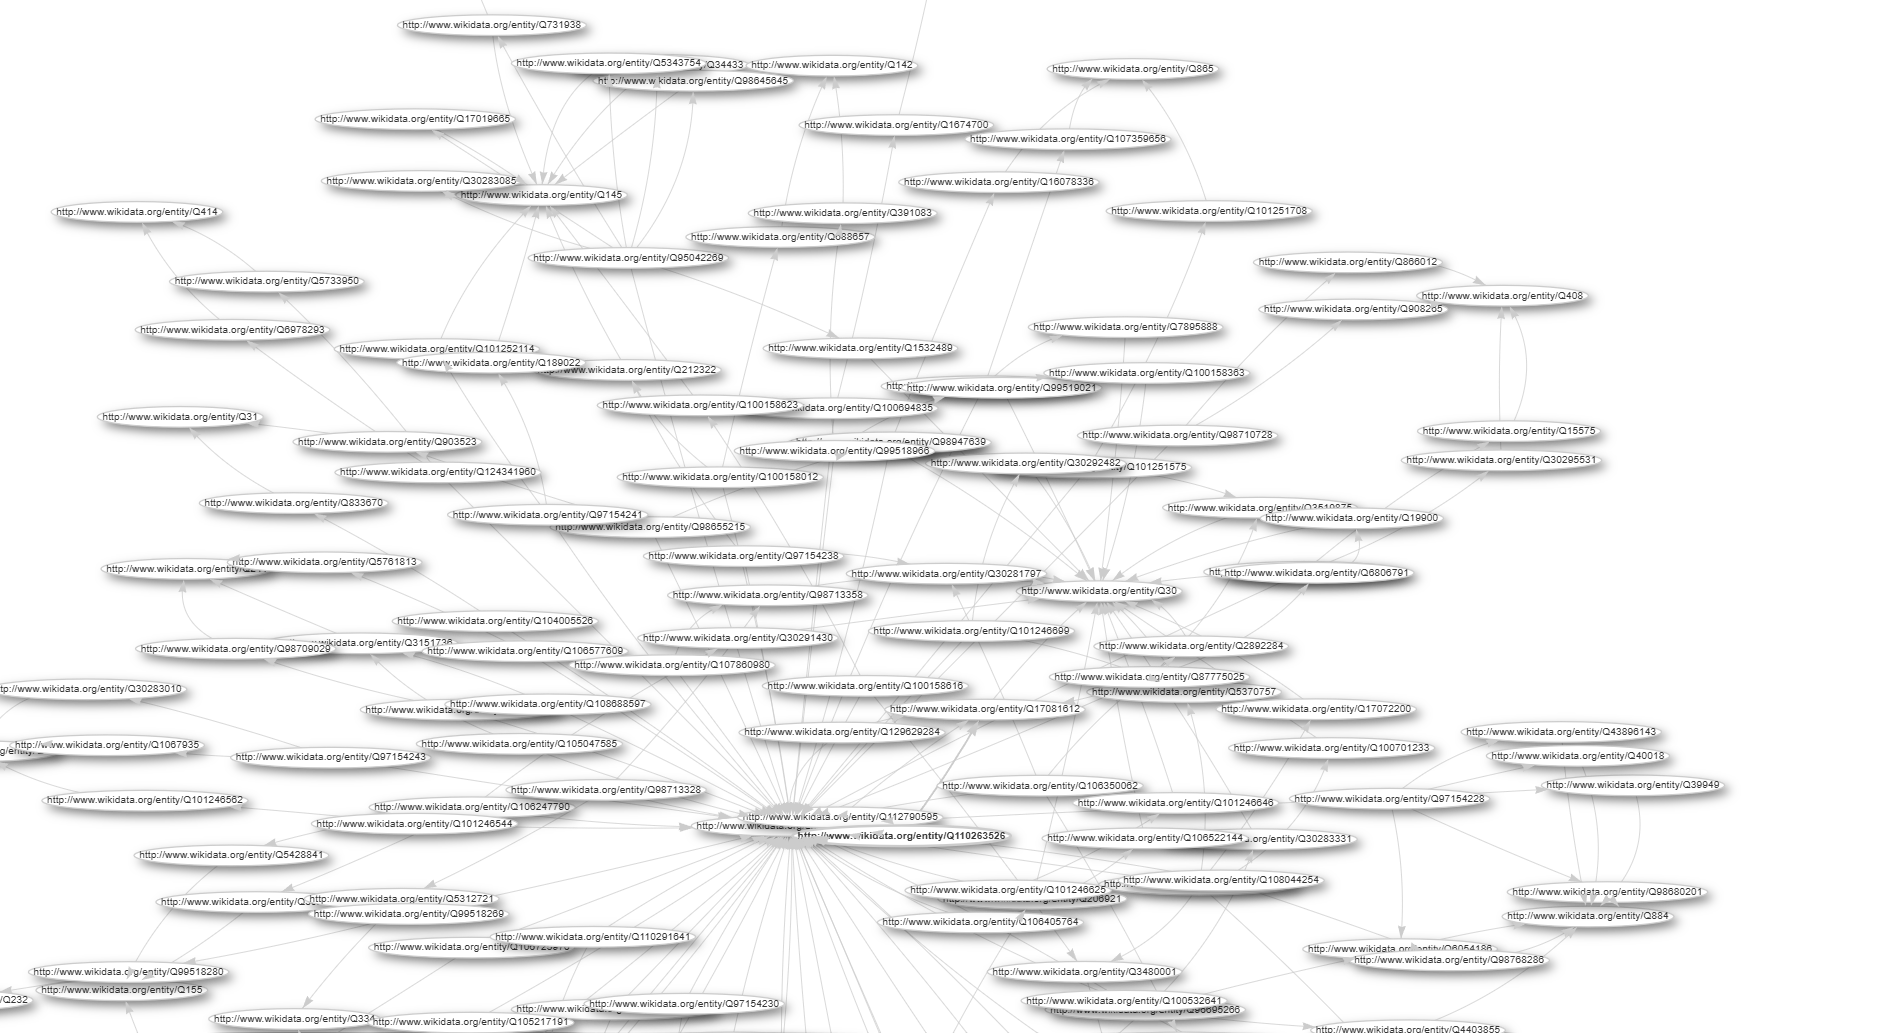
\includegraphics[width=0.8\textwidth]{download.png}
  \caption{RDF graph visualization of vaccine--developer--country relationships
           returned by the \texttt{CONSTRUCT} query in Listing~\ref{lst:q3construct_visual}.}
  \label{fig:q2graph}
\end{figure}

% ══════════════════════════════════════════════════════════════════════════════
\newpage
\section{Discussion}
\label{sec:discussion}

\subsection{Benefits of Linked Data}
\begin{itemize}
  \item \textbf{Federated access}: a single SPARQL query can join data from
        UniProt, Bgee, and GO without pre-downloading or merging the datasets.
  \item \textbf{Open standards}: RDF and SPARQL are W3C standards, ensuring
        interoperability and long-term stability.
  \item \textbf{Provenance}: \texttt{CONSTRUCT} queries make justification
        first-class, enabling auditability.
  \item \textbf{Precision}: results are exact matches to the query, not
        probabilistic generations.
\end{itemize}

\subsection{Limitations of Linked Data}
\begin{itemize}
  \item \textbf{Steep learning curve}: formulating correct SPARQL queries
        requires knowledge of the target ontologies and data models.
  \item \textbf{Endpoint fragility}: federated queries fail if any remote
        endpoint is unavailable or slow.
  \item \textbf{Data completeness}: Wikidata and other community-driven
        graphs may have missing or inconsistent entries.
  \item \textbf{No reasoning over free text}: Linked Data cannot interpret
        documents, images, or unstructured annotations without additional NLP.
\end{itemize}

\subsection{Benefits and limitations of the hybrid approach}

The hybrid pipeline inherits the benefits of both paradigms: the accessibility
of LLMs and the precision and provenance of Linked Data.
Its main limitation is error propagation: an incorrectly generated SPARQL query
(hallucinated property names, wrong class URIs) will produce wrong or empty
results with no obvious error message for the end user.
Human-in-the-loop validation at the query generation step is therefore
essential.

% ══════════════════════════════════════════════════════════════════════════════
\newpage
\section{Conclusion}
\label{sec:conclusion}

This project demonstrated that the Semantic Web stack remains uniquely suited
for answering complex, cross-domain factual questions that require structured,
live, and justified data retrieval.
Federated SPARQL queries, spanning UniProt, Bgee, and Wikidata, provide answers
that LLMs cannot reliably generate from training data alone.
The \texttt{CONSTRUCT} mechanism adds formal explainability, a critical feature
for scientific and high-stakes applications.
Finally, the hybrid Linked Data + LLM pipeline offers a pragmatic path forward:
LLMs lower the barrier to query formulation, while Linked Data guarantees
accuracy, freshness, and provenance.

% ══════════════════════════════════════════════════════════════════════════════
\newpage
\begin{thebibliography}{9}

\bibitem{bernerslee2001}
T.~Berners-Lee, J.~Hendler, and O.~Lassila,
``The Semantic Web,''
\textit{Scientific American}, vol.~284, no.~5, pp.~34--43, 2001.

\bibitem{tbl2009}
T.~Berners-Lee,
``The Next Web'' (TED Talk), 2009.
\url{https://www.ted.com/talks/tim_berners_lee_the_next_web}

\bibitem{lodcloud}
M.~Schmachtenberg, C.~Bizer, and H.~Paulheim,
``Adoption of the Linked Data Best Practices in Different Topical Domains,''
in \textit{Proc. ISWC}, 2014.
\url{https://lod-cloud.net}

\bibitem{sparql11}
S.~Harris, A.~Seaborne, et al.,
``SPARQL 1.1 Query Language,'' W3C Recommendation, March 2013.
\url{https://www.w3.org/TR/sparql11-query/}

\bibitem{uniprot}
UniProt Consortium,
``UniProt: the Universal Protein Knowledgebase in 2023,''
\textit{Nucleic Acids Research}, vol.~51, D1, pp.~D523--D531, 2023.
\url{https://sparql.uniprot.org/sparql}

\bibitem{bgee}
F.~Bastian et al.,
``Bgee in 2023: Improved coverage and new features for gene expression
data in animals,''
\textit{Nucleic Acids Research}, vol.~51, D1, pp.~D1951--D1958, 2023.
\url{https://www.bgee.org/sparql}

\bibitem{wikidata}
D.~Vrandecic and M.~Krötzsch,
``Wikidata: A Free Collaborative Knowledgebase,''
\textit{Communications of the ACM}, vol.~57, no.~10, pp.~78--85, 2014.
\url{https://query.wikidata.org}

\bibitem{linkedlifedata}
Ontotext,
``Linked Life Data,''
\url{https://linkedlifedata.com}, 2023.

\end{thebibliography}

\end{document}
